\documentclass{standalone}
\usepackage{tikz}
\usepackage{amsmath}

\begin{document}

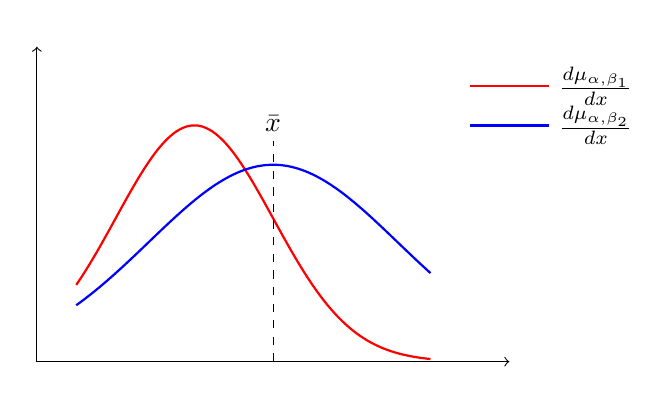
\begin{tikzpicture}
    % Define styles for the curves
    \draw[->] (0,0) -- (6,0) node[right] {};
    \draw[->] (0,0) -- (0,4) node[above] {};

    % Red curve
    \draw[red, thick] plot[domain=0.5:5, samples=100] (\x, {3*exp(-0.5*(\x-2)^2)});
    
    % Blue curve
    \draw[blue, thick] plot[domain=0.5:5, samples=100] (\x, {2.5*exp(-0.2*(\x-3)^2)});
    
    % Dashed line at x-bar
    \draw[dashed] (3,0) -- (3,2.8) node[above] {$\bar{x}$};

    % Legend
    \draw[red, thick] (5.5,3.5) -- (6.5,3.5) node[right, black] {$\frac{d\mu_{\alpha, \beta_1}}{dx}$};
    \draw[blue, thick] (5.5,3) -- (6.5,3) node[right, black] {$\frac{d\mu_{\alpha, \beta_2}}{dx}$};
\end{tikzpicture}

\end{document}